% Options for packages loaded elsewhere
\PassOptionsToPackage{unicode}{hyperref}
\PassOptionsToPackage{hyphens}{url}
%
\documentclass[
]{article}
\usepackage{amsmath,amssymb}
\usepackage{lmodern}
\usepackage{iftex}
\ifPDFTeX
  \usepackage[T1]{fontenc}
  \usepackage[utf8]{inputenc}
  \usepackage{textcomp} % provide euro and other symbols
\else % if luatex or xetex
  \usepackage{unicode-math}
  \defaultfontfeatures{Scale=MatchLowercase}
  \defaultfontfeatures[\rmfamily]{Ligatures=TeX,Scale=1}
\fi
% Use upquote if available, for straight quotes in verbatim environments
\IfFileExists{upquote.sty}{\usepackage{upquote}}{}
\IfFileExists{microtype.sty}{% use microtype if available
  \usepackage[]{microtype}
  \UseMicrotypeSet[protrusion]{basicmath} % disable protrusion for tt fonts
}{}
\makeatletter
\@ifundefined{KOMAClassName}{% if non-KOMA class
  \IfFileExists{parskip.sty}{%
    \usepackage{parskip}
  }{% else
    \setlength{\parindent}{0pt}
    \setlength{\parskip}{6pt plus 2pt minus 1pt}}
}{% if KOMA class
  \KOMAoptions{parskip=half}}
\makeatother
\usepackage{xcolor}
\usepackage[margin=1in]{geometry}
\usepackage{graphicx}
\makeatletter
\def\maxwidth{\ifdim\Gin@nat@width>\linewidth\linewidth\else\Gin@nat@width\fi}
\def\maxheight{\ifdim\Gin@nat@height>\textheight\textheight\else\Gin@nat@height\fi}
\makeatother
% Scale images if necessary, so that they will not overflow the page
% margins by default, and it is still possible to overwrite the defaults
% using explicit options in \includegraphics[width, height, ...]{}
\setkeys{Gin}{width=\maxwidth,height=\maxheight,keepaspectratio}
% Set default figure placement to htbp
\makeatletter
\def\fps@figure{htbp}
\makeatother
\setlength{\emergencystretch}{3em} % prevent overfull lines
\providecommand{\tightlist}{%
  \setlength{\itemsep}{0pt}\setlength{\parskip}{0pt}}
\setcounter{secnumdepth}{-\maxdimen} % remove section numbering
\usepackage{booktabs}
\usepackage{longtable}
\usepackage{array}
\usepackage{multirow}
\usepackage{wrapfig}
\usepackage{float}
\usepackage{colortbl}
\usepackage{pdflscape}
\usepackage{tabu}
\usepackage{threeparttable}
\usepackage{threeparttablex}
\usepackage[normalem]{ulem}
\usepackage{makecell}
\usepackage{xcolor}
\ifLuaTeX
  \usepackage{selnolig}  % disable illegal ligatures
\fi
\IfFileExists{bookmark.sty}{\usepackage{bookmark}}{\usepackage{hyperref}}
\IfFileExists{xurl.sty}{\usepackage{xurl}}{} % add URL line breaks if available
\urlstyle{same} % disable monospaced font for URLs
\hypersetup{
  pdftitle={Generación de energía},
  pdfauthor={Escuela Colombiana de Ingeniería Julio Garavito},
  hidelinks,
  pdfcreator={LaTeX via pandoc}}

\title{Generación de energía}
\author{Escuela Colombiana de Ingeniería Julio Garavito}
\date{2023-03-28}

\begin{document}
\maketitle

\textbf{Incluir:} una explicación de la diferencia entre relaciones
entre variables y relaciones entre individuos.

\hypertarget{temas-a-tratar}{%
\subsection{Temas a tratar}\label{temas-a-tratar}}

\begin{itemize}
\item
  Introducción al análisis estadístico multivariado
\item
  Distancias en el análisis estadístico multivariado
\item
  Distancias con variables cualitativas
\item
  Distancias con variables cuantitativas
\item
  Conclusiones Generales
\end{itemize}

\hypertarget{analisis-estadistico-multivariado}{%
\subsection{Analisis estadistico
multivariado}\label{analisis-estadistico-multivariado}}

El análisis estadístico multivariado es una técnica que permite analizar
conjuntos de datos que involucran múltiples variables, estudiando cómo
se relacionan entre sí y cómo afectan conjuntamente a un resultado o
variable de interés mediante el uso de diversas técnicas estadísticas.

\hypertarget{distancias-en-el-anuxe1lisis-estaduxedstico-multivariado}{%
\subsection{Distancias en el análisis estadístico
multivariado}\label{distancias-en-el-anuxe1lisis-estaduxedstico-multivariado}}

\begin{itemize}
\tightlist
\item
  En el análisis estadístico multivariado, se trabaja con múltiples
  variables.
\item
  Las distancias son una medida de la similitud o diferencia entre los
  objetos (individuos, variables, etc.) en función de estas variables.
\item
  Son ampliamente utilizadas en análisis de datos, clusterización,
  clasificación, entre otros.
\item
  En esta presentación, nos enfocaremos en algunas de las distancias más
  utilizadas en el análisis estadístico multivariado.
\end{itemize}

\hypertarget{selecciuxf3n-de-la-medida-de-distancia-en-anuxe1lisis-estaduxedstico-multivariado}{%
\subsection{Selección de la medida de distancia en análisis estadístico
multivariado}\label{selecciuxf3n-de-la-medida-de-distancia-en-anuxe1lisis-estaduxedstico-multivariado}}

\begin{itemize}
\tightlist
\item
  La elección de la medida de distancia adecuada depende del objetivo
  del análisis.
\item
  Depende del tipo de datos y de la escala de medida de las variables.
\item
  La elección también puede depender de la estructura de los datos (por
  ejemplo, si hay datos faltantes o valores extremos).
\item
  Es importante tener en cuenta las propiedades de las medidas de
  distancia, como la simetría, la triangularidad y la identidad de los
  indiscernibles.
\end{itemize}

\hypertarget{selecciuxf3n-de-la-medida-de-distancia-en-anuxe1lisis-estaduxedstico-multivariado-1}{%
\subsection{Selección de la medida de distancia en análisis estadístico
multivariado}\label{selecciuxf3n-de-la-medida-de-distancia-en-anuxe1lisis-estaduxedstico-multivariado-1}}

\begin{itemize}
\tightlist
\item
  Si el objetivo es encontrar grupos de objetos similares, se pueden
  utilizar medidas de distancia que enfaticen la similitud, como la
  distancia euclidiana.
\item
  Si el objetivo es clasificar objetos en diferentes categorías, se
  pueden utilizar medidas de distancia que minimicen la variabilidad
  dentro de cada categoría, como la distancia de Mahalanobis.
\item
  Si el objetivo es determinar la estructura subyacente de los datos, se
  pueden utilizar medidas de distancia que revelen patrones de
  covariación entre las variables, como la distancia de correlación.
\item
  Si el objetivo es identificar objetos anómalos o extremos, se pueden
  utilizar medidas de distancia robustas, como la distancia de Minkowski
  con un valor de p mayor que 1.
\end{itemize}

\hypertarget{medidas-de-distancia-entre-individuos}{%
\subsection{Medidas de distancia entre
individuos}\label{medidas-de-distancia-entre-individuos}}

\begin{itemize}
\item
  La elección de la medida de distancia entre individuos puede depender
  de la escala de medida de las variables y del tipo de variables.
\item
  Si las variables están en diferentes escalas, la distancia euclidiana
  no será adecuada ya que una variable con una escala más grande tendrá
  una mayor influencia en la medida de distancia.
\item
  Si las variables son de tipo categórico o nominal, la distancia
  euclidiana no se puede utilizar y se deben usar medidas de distancia
  apropiadas para variables categóricas, como la distancia de Gower.
\item
  Si las variables son de tipo ordinal, la distancia euclidiana no es la
  mejor medida y se pueden utilizar medidas de distancia apropiadas para
  variables ordinales, como la distancia de Spearman.
\item
  Si las variables son de tipo binario, se puede utilizar la distancia
  de Hamming.
\item
  Si las variables son mixtas (numéricas y categóricas), se pueden
  utilizar medidas de distancia apropiadas para datos mixtos, como la
  distancia de Gower.
\item
  Si las variables están en diferentes escalas, se pueden utilizar
  medidas de distancia que tengan en cuenta la variabilidad y la escala
  de cada variable, como la distancia de Mahalanobis.
\end{itemize}

\hypertarget{medidas-de-distancia-entre-variables}{%
\subsection{Medidas de distancia entre
variables}\label{medidas-de-distancia-entre-variables}}

\begin{itemize}
\tightlist
\item
  La elección de la medida de distancia entre variables también puede
  depender de la escala de medida y del tipo de variables.
\end{itemize}

\hypertarget{distancias-con-variables-cualitativas}{%
\subsection{Distancias con variables
cualitativas}\label{distancias-con-variables-cualitativas}}

En el análisis multivariado de variables cualitativas, la distancia se
refiere a la medida de la diferencia entre dos observaciones o
individuos en función de sus características o variables cualitativas.
Existen diferentes medidas de distancia que se pueden utilizar en el
análisis multivariado de variables cualitativas. Algunas de las más
comunes son:

\begin{itemize}
\item
  Distancia Hamming
\item
  Distancia Jaccard
\end{itemize}

\hypertarget{distancia-hamming}{%
\subsection{Distancia Hamming}\label{distancia-hamming}}

La distancia de Hamming es una medida de la distancia entre dos cadenas
de igual longitud. La fórmula para calcular la distancia de Hamming es
la siguiente:

\[ D_H(x, y) = \sum_{i=1}^{n} \mathbb{I}(x_i \neq y_i) \] Donde \(x\) y
\(y\) son las cadenas que se van a comparar, \(n\) es la longitud de las
cadenas y \(\mathbb{I}(x_i \neq y_i)\) es una función indicadora que
devuelve 1 si los caracteres en las posiciones \(i\) de \(x\) y \(y\)
son diferentes y 0 en caso contrario.

\hypertarget{ejemplo}{%
\subsection{Ejemplo}\label{ejemplo}}

Supongamos que tenemos dos cadenas binarias de la misma longitud, x =
``0110101'' e y = ``1100110''. Queremos calcular la distancia de Hamming
entre estas dos cadenas.

Para ello, podemos utilizar la fórmula anterior,

\[D_H(x, y) = \sum_{i=1}^7 \mathbb{I}(x_i \neq y_i)\]

\[D_H(x, y) = \mathbb{I}(0 \neq 1) + \mathbb{I}(1 \neq 1) + \mathbb{I}(1 \neq 0) + \mathbb{I}(0 \neq 0) + \mathbb{I}(1 \neq 0) + \mathbb{I}(0 \neq 1) + \mathbb{I}(1 \neq 0)\]

\[D_H(x, y) = 1 + 0 + 1 + 0 + 1 + 1 + 1\]

Por lo tanto, la distancia de Hamming entre las cadenas binarias x e y
es de 5. Esto significa que hay 5 posiciones en las que las cadenas
difieren.

\hypertarget{distancia-jaccard}{%
\subsection{Distancia Jaccard}\label{distancia-jaccard}}

Se utiliza para medir la similitud entre dos conjuntos de variables
cualitativas.

La distancia de Jaccard entre dos conjuntos \(A\) y \(B\) se define
como:

\[ d_J(A,B) = 1 - \frac{|A \cap B|}{|A \cup B|} \]

Donde \(|A|\) representa el tamaño del conjunto \(A\) y \(A \cap B\) y
\(A \cup B\) representan la intersección y la unión de los conjuntos
\(A\) y \(B\), respectivamente. Esta fórmula mide la distancia entre dos
conjuntos basándose en la similitud entre ellos.

\hypertarget{ejemplo-1}{%
\subsection{Ejemplo}\label{ejemplo-1}}

A continuación, se presenta una tabla que contiene información acerca de
los clientes y los productos adquiridos. En dicha tabla, se representa
con el número 0 cuando el cliente no ha comprado el producto y con el
número 1 cuando sí lo ha adquirido.

\hypertarget{ejemplo-2}{%
\subsection{Ejemplo}\label{ejemplo-2}}

Con base en los datos recolectados previamente, se realiza el cálculo de
la distancia Jaccard entre cada cliente, con el fin de identificar
patrones y tendencias en su comportamiento y asi tener una tomar
decisiones más precisas e informadas. El resultado de este cálculo se
producirá en una matriz de distancias, que sintetizará de manera
efectiva los resultados obtenidos.

\hypertarget{conclusiones}{%
\subsection{Conclusiones}\label{conclusiones}}

\begin{itemize}
\item
  Los clientes cuyas distancias son más cercanas a 0 tienen un alto
  grado de similitud en sus compras. tal es el caso de los clientes A y
  B, C y D que presentan una distancia de 0,33 lo que indica que tienen
  patrones de compra similares.
\item
  Los clientes que tienen una distancia de 0,50 como los clientes B y D,
  tienen una afinidad del 50\% en sus compras. Esto significa que
  dividen la mitad de los productos que compran.
\item
  Los clientes cuyas distancias son más cercanas a 1 tienen un alto
  grado de disimilitud en sus compras, como lo son, los clientes A y D,
  asi como los clientes B y C que presentan una distancia de 0,75 Esta
  medida indica que estos clientes presentan la mayor disimilitud entre
  todos los datos analizados en cuanto a sus patrones de compra.
\end{itemize}

\hypertarget{distancias-con-variables-cuantitativas}{%
\subsection{Distancias con variables
cuantitativas}\label{distancias-con-variables-cuantitativas}}

En análisis multivariado, se utilizan diferentes métodos para medir la
distancia entre observaciones con variables cuantitativas. Estas medidas
de distancia son utilizadas en técnicas como análisis de componentes
principales, análisis de correspondencias, análisis de conglomerados,
entre otras.

A continuación, se describen algunas de las medidas de distancia más
comunes en análisis multivariado con variables cuantitativas:

\begin{itemize}
\item
  Distancia Euclidiana
\item
  Distancia Manhattan
\item
  Distancia Mahalanobis
\end{itemize}

\hypertarget{distancia-euclidiana}{%
\subsection{Distancia Euclidiana}\label{distancia-euclidiana}}

La distancia euclidiana es una medida de la distancia entre dos puntos
en un espacio euclidiano de dos o más dimensiones.

La distancia euclidiana entre dos puntos \(p\) y \(q\) en un espacio
euclidiano de \(n\) dimensiones se define como:

\[ d_E(p,q) = \sqrt{\sum_{i=1}^{n} (p_i - q_i)^2} \]

Donde \(p_i\) y \(q_i\) son las coordenadas del punto \(p\) y el punto
\(q\) en la \(i\)-ésima dimensión, respectivamente.

\hypertarget{ejemplo-3}{%
\subsection{Ejemplo}\label{ejemplo-3}}

Supongamos que tenemos dos vectores P y Q:

\(p = (1, 2, 3)\) y \(q = (4, 5, 6)\), entonces la distancia euclidiana
entre \(p\) y \(q\) es:

\[ d_E(p,q) = \sqrt{(1-4)^2 + (2-5)^2 + (3-6)^2} = \sqrt{27} \approx 5.196 \]

\hypertarget{distancia-manhattan}{%
\subsection{Distancia Manhattan}\label{distancia-manhattan}}

La distancia de Manhattan es una medida de distancia entre dos puntos en
un espacio euclidiano de n dimensiones, mide la distancia que hay que
recorrer para ir de un punto a otro si sólo se permiten movimientos en
línea recta horizontal o vertical.La fórmula para calcular la distancia
de Manhattan es la siguiente:

\[ D_M(x, y) = \sum_{i=1}^{n} |x_i - y_i| \]

Donde \(x\) y \(y\) son los vectores que se van a comparar, \(n\) es el
número de dimensiones y \(|x_i - y_i|\) representa la diferencia
absoluta entre la coordenada \(i\) de \(x\) y la coordenada \(i\) de
\(y\).

\hypertarget{ejemplo-4}{%
\subsection{Ejemplo}\label{ejemplo-4}}

Supongamos que tenemos dos vectores X y Y:

\(x = (1, 2, 3)\) y \(y = (4, 5, 6)\), entonces la distancia Manhattan
entre \(x\) y \(y\) es:

\[ D_M(x) = |1 - 4| + |2 - 5| + |3 - 6| = 9 \]

\hypertarget{distancia-mahalanobis}{%
\subsection{Distancia Mahalanobis}\label{distancia-mahalanobis}}

La distancia de Mahalanobis es una medida de la distancia entre un punto
y un conjunto de puntos, teniendo en cuenta la covarianza entre las
variables. La fórmula para calcular la distancia de Mahalanobis es la
siguiente:

\[ D_M(x) = \sqrt{(x - \mu)^T \Sigma^{-1} (x - \mu)} \]

Donde \(x\) es el vector de variables, \(\mu\) es el vector de medias y
\(\Sigma\) es la matriz de covarianza.

Donde \(p_i\) y \(q_i\) son las coordenadas del punto \(p\) y el punto
\(q\) en la \(i\)-ésima dimensión, respectivamente.

\hypertarget{ejemplo-5}{%
\subsection{Ejemplo}\label{ejemplo-5}}

En el siguiente ejemplo se utiliza la distancia de Mahalanobis para
detectar valores atípicos en un conjunto de datos simulado de
características de televisores. lo que puede ayudar a detectar problemas
en la producción o a tomar decisiones de marketing y precios más
informadas.

\begin{verbatim}
##   resolucion_pantalla consumo_energia precio distancia_maha
## 1                1593              57    700       3.068845
## 2                1110             197   1500       2.806825
## 3                1846             217   1000       2.725497
## 4                1139             170   3000       2.543593
## 5                1856              80    500       1.464287
## 6                1529             219   1200       1.401068
\end{verbatim}

\hypertarget{conclusiones-1}{%
\subsection{Conclusiones}\label{conclusiones-1}}

Al analizar detalladamente la tabla anterior, podemos concluir que
aquellos dispositivos tecnológicos que se encuentran significativamente
alejados de la media podrían estar experimentando problemas relacionados
con sus características. Por el contrario, aquellos dispositivos que se
encuentran en posiciones más cercanas a la media sugieren una mayor
estabilidad en sus características.

Por consiguiente, los fabricantes de dispositivos electrónicos deben
considerar cuidadosamente estos resultados al diseñar y promocionar sus
productos, con el fin de optimizar su posicionamiento en el mercado y
ofrecer el mejor valor a sus clientes.

\hypertarget{diagrama-de-dispersion}{%
\subsection{Diagrama de dispersion}\label{diagrama-de-dispersion}}

A continuación, se presenta un gráfico que permite una mejor
visualización de la relación entre las variables, lo que facilita la
identificación de patrones y tendencias en los datos.

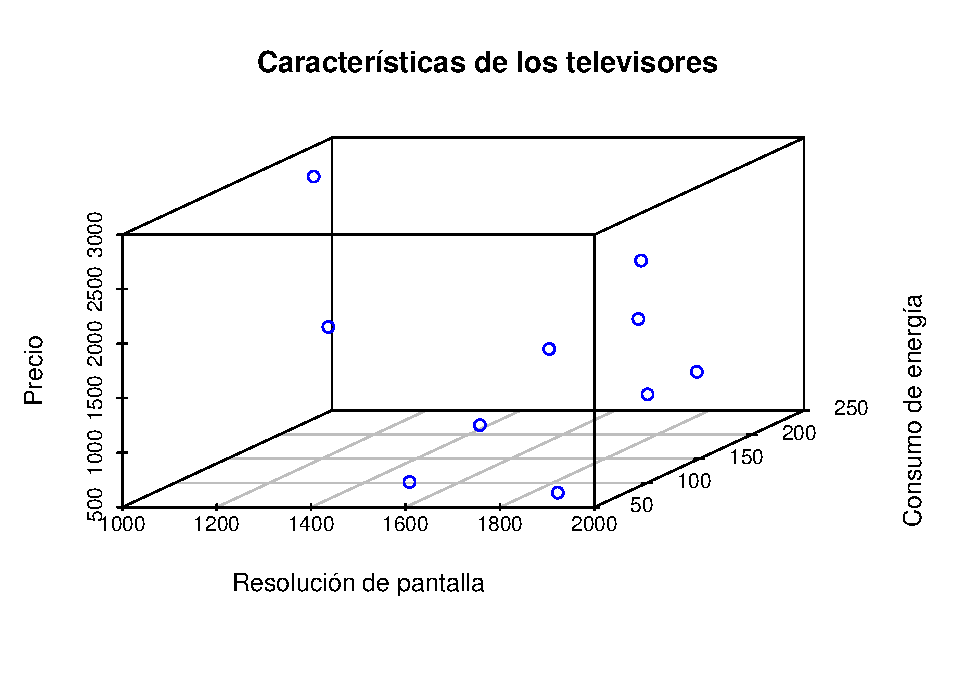
\includegraphics{AMTV_Docum_Consolidado_files/figure-latex/scatterplot3d-1.pdf}

\hypertarget{conclusiones-2}{%
\subsection{Conclusiones}\label{conclusiones-2}}

\begin{itemize}
\item
  Resolución de pantalla y precio: se puede observar una relación
  positiva entre la resolución de pantalla y el precio de los
  televisores. Esto sugiere que los televisores con una resolución de
  pantalla más alta tienden a tener un precio más alto.
\item
  Consumo de energía y precio: se puede observar una relación negativa
  entre el consumo de energía y el precio de los televisores. Esto
  sugiere que los televisores que consumen menos energía tienden a tener
  un precio más alto.
\item
  Distancia entre los puntos: la distancia entre los puntos en la
  gráfica indica la similitud en las características de los televisores.
  Por ejemplo, los televisores con una resolución de pantalla similar y
  un consumo de energía similar tienden a estar más cerca de unos de
  otros.
\item
  Dos grupos claros: se puede observar que hay dos grupos claros de
  televisores en la gráfica: uno con una resolución de pantalla alta y
  un consumo de energía bajo, y otro con una resolución de pantalla más
  baja y un consumo de energía más alto.
\end{itemize}

\hypertarget{tabla}{%
\subsection{Tabla}\label{tabla}}

A continuacion, se presenta una tabla sintetizada que resume las
distancias y sus respectivos tipos, es decir, si aplica para variables
cualitativo o cuantitativo

\begin{verbatim}
## # A tibble: 2 x 6
##   Tipos        Hamming Jaccard Euclidiana Manhattan Mahalanobis
##   <chr>        <chr>   <chr>   <chr>      <chr>     <chr>      
## 1 Cualitativo  "OK"    "OK"    ""         ""        ""         
## 2 Cuantitativo ""      ""      "OK"       "OK"      "OK"
\end{verbatim}

\hypertarget{conclusiones-generales}{%
\subsection{Conclusiones Generales}\label{conclusiones-generales}}

En el análisis multivariado, el uso de medidas de distancia como la
Hamming, Jaccard, Euclidiana, Manhatan y Mahalanobis es esencial para
comprender la estructura de los datos y las relaciones entre las
variables.

\begin{itemize}
\item
  La distancia Hamming es útil para medir la distancia entre dos
  secuencias de datos binarios.
\item
  La distancia de Jaccard es adecuada para datos categóricos.
\item
  La distancia euclidiana es muy utilizada en el análisis de datos
  numéricos y es fácil de interpretar.
\item
  La distancia de Manhattan es una alternativa útil cuando los datos
  tienen una alta dimensionalidad.
\item
  La distancia de Mahalanobis tiene en cuenta la conexión entre las
  variables y es adecuada para datos multivariados.
\end{itemize}

En resumen, la selección de la medida de distancia adecuada para el
análisis multivariado depende tanto de la naturaleza de los datos como
del objetivo de dicho análisis. Cabe destacar que las distancias
mencionadas anteriormente son sólo algunas de las muchas disponibles en
el ámbito del analisis estadístico multivariado.

\hypertarget{aplicacion}{%
\subsection{Aplicacion}\label{aplicacion}}

La generación de energía se refiere al proceso de producir la cantidad
necesaria de energía para satisfacer las necesidades de la sociedad.
Esta energía puede adoptar diversas formas, como electricidad, calor,
combustibles líquidos o gaseosos, entre otras. Para llevar a cabo este
proceso se utilizan diferentes fuentes de energía primaria, como el
petróleo, el gas natural, el carbón, la energía nuclear, la energía
hidroeléctrica, la energía solar, la energía eólica, entre otras. La
elección de la fuente depende de varios factores, como la
disponibilidad, la accesibilidad, la tecnología y la regulación. La
generación de energía es esencial para la sociedad moderna, ya que
permite realizar actividades cotidianas como iluminar hogares,
transportar personas y bienes, procesar alimentos y producir bienes y
servicios. Sin embargo, también puede tener impactos significativos en
el medio ambiente y en la sociedad, como la emisión de gases de efecto
invernadero, la contaminación del aire y del agua, y la alteración de
ecosistemas naturales.

Partiendo de la información anterior, se llevó a cabo un análisis
multivariado que involucró a 141 países y 12 formas de generación de
energía. El objetivo fue mostrar cómo cada país genera energía, teniendo
en cuenta las siguientes formas de generación:

\begin{verbatim}
##                 V1   Coal    Oil    Gas Biofuels Waste Nuclear Hydro Geothermal
##  1:        Albania      0      0      0        0     0       0  5895          0
##  2:       Alemania 283710   6209  63017    44555 12824   91786 24898        134
##  3:        Algeria      0    908  67668        0     0       0   145          0
##  4:         Angola      0   4572      0        0     0       0  5193          0
##  5: Arabia Saudita      0 149537 188804        0     0       0     0          0
##  6:      Argentina   3303  22357  71367     2138     0    7139 38529          0
##  7:        Armenia      0      0   2801        0     0    2788  2206          0
##  8:      Australia 158610   6799  52462     3608     0       0 13445          1
##  9:        Austria   5081    861   7783     4121  1069       0 40592          0
## 10:     Azerbaijan      0   1607  21252        0   182       0  1637          0
## 11:     Bangladesh    997   9666  47624        0     0       0   566          0
##     Solar PV Solar thermal  Wind Tide
##  1:        0             0     0    0
##  2:    38726             0 79206    0
##  3:       58             0    19    0
##  4:        0             0     0    0
##  5:        1             0     0    0
##  6:       15             0   599    0
##  7:        1             0     3    0
##  8:     5019             4 11467    0
##  9:      937             0  4840    0
## 10:        5             0     5    0
## 11:      154             0     4    0
\end{verbatim}

\begin{itemize}
\tightlist
\item
  Carbón:La generación de energía con carbón implica la quema del carbón
  en una caldera para producir vapor que mueve una turbina y genera
  electricidad. Este proceso es altamente contaminante ya que emite
  grandes cantidades de dióxido de carbono y otros contaminantes,
  contribuyendo significativamente al cambio climático y teniendo
  efectos negativos en la salud y el medio ambiente.
\end{itemize}

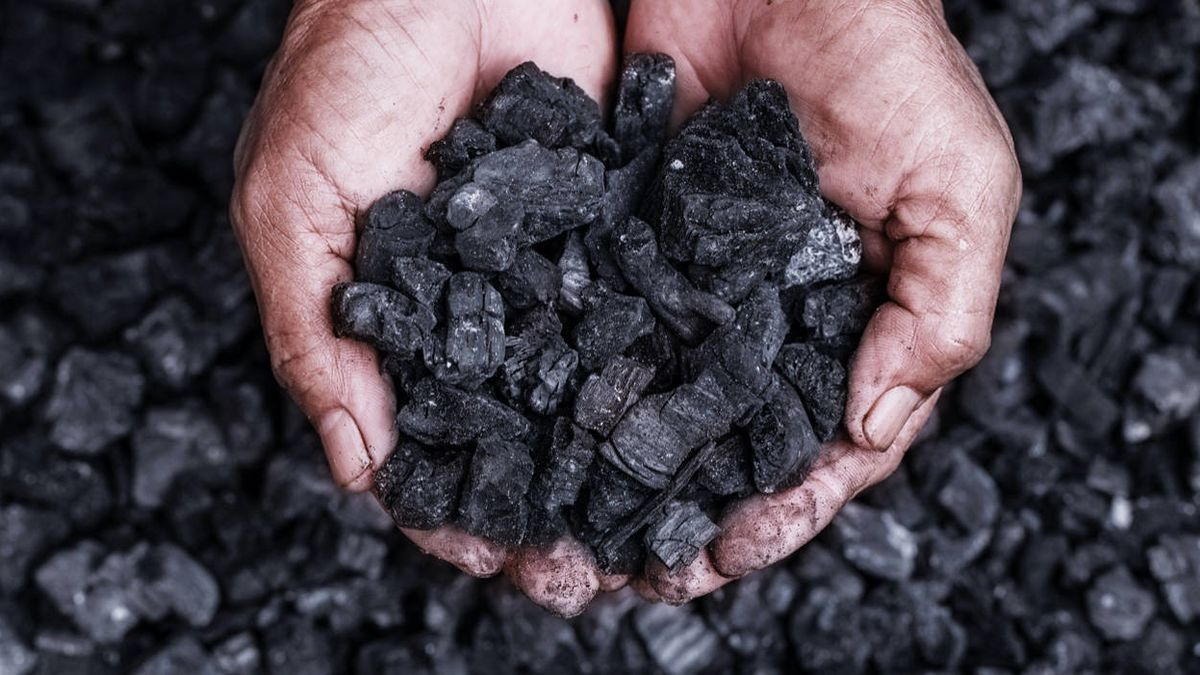
\includegraphics[width=4.16667in,height=\textheight]{carbon.jpeg}

\begin{itemize}
\tightlist
\item
  Aceite:La generación de energía con aceite implica la quema del
  combustible líquido en una caldera para producir vapor que mueve una
  turbina y genera electricidad. Aunque es menos contaminante que la
  generación de energía con carbón, aún produce emisiones de gases de
  efecto invernadero y otros contaminantes que pueden tener efectos
  negativos en la salud y el medio ambiente.
\end{itemize}

\usepackage{floatrow}
\floatsetup[figure]{capposition=top}

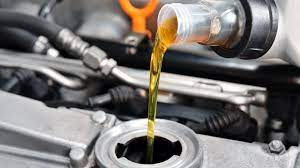
\includegraphics[width=4.16667in,height=\textheight]{aceite.jpeg}

\begin{itemize}
\tightlist
\item
  Gas:La generación de energía con gas implica la quema de gas natural
  en una central eléctrica para producir electricidad. El gas natural se
  extrae de yacimientos subterráneos y se transporta a través de
  tuberías hasta la central eléctrica. Allí, el gas se quema en una
  turbina o en una caldera para producir vapor que mueve una turbina y
  genera electricidad. La generación de energía con gas natural es una
  alternativa más limpia que la generación de energía con carbón o
  petróleo, ya que produce menos emisiones de gases de efecto
  invernadero y otros contaminantes. Además, el gas natural es una
  fuente de energía relativamente abundante y fácil de transportar, lo
  que lo convierte en una opción popular para la generación de
  electricidad.
\end{itemize}

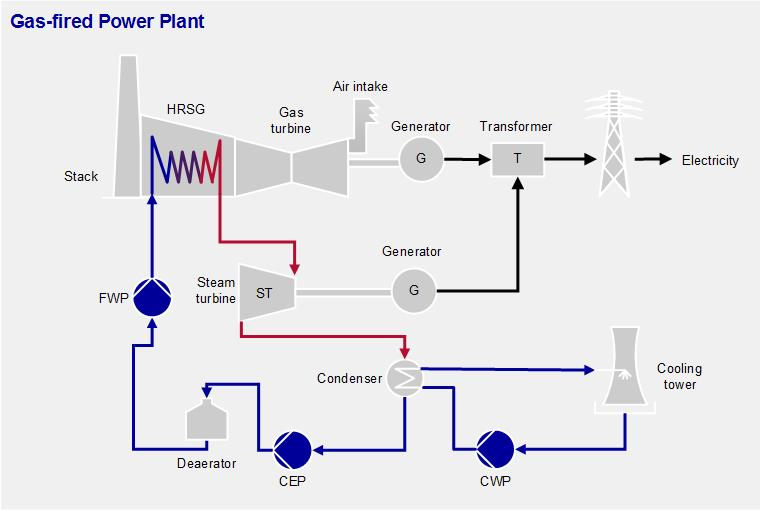
\includegraphics[width=4.16667in,height=\textheight]{gas.jpeg}

\begin{itemize}
\tightlist
\item
  Biocombustibles:La generación de energía con biocombustibles implica
  el uso de materiales orgánicos, como madera, cultivos energéticos,
  residuos de la agricultura o de la industria alimentaria, y otros
  residuos biodegradables para producir electricidad. En este proceso,
  los materiales orgánicos se queman en una caldera para producir vapor
  que mueve una turbina y genera electricidad. Los biocombustibles son
  una alternativa más sostenible y renovable a los combustibles fósiles,
  ya que su producción y uso emiten menos gases de efecto invernadero y
  otros contaminantes. Además, el uso de biocombustibles puede ayudar a
  reducir la cantidad de residuos orgánicos que van a los vertederos y
  contribuyen a la contaminación del suelo y el agua.
\end{itemize}

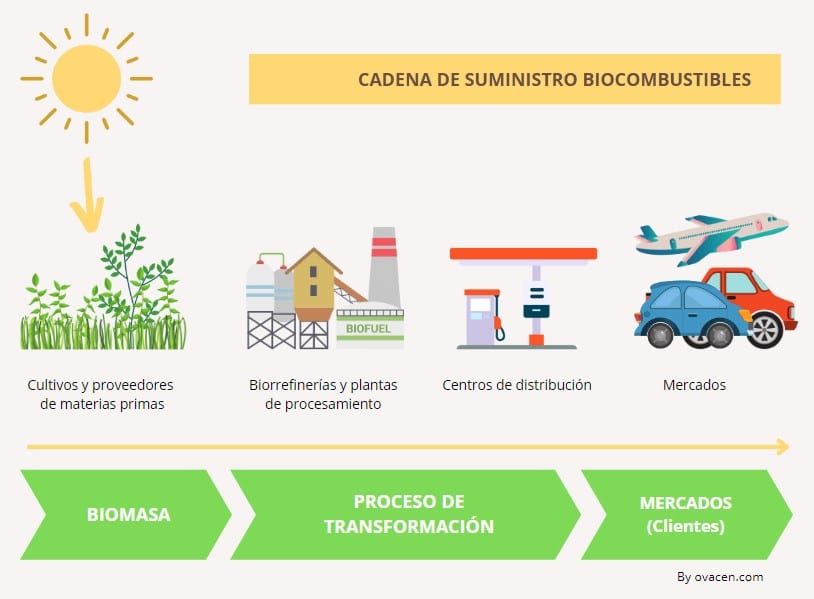
\includegraphics[width=4.16667in,height=\textheight]{bio.jpeg}

\begin{itemize}
\tightlist
\item
  Desperdicios:La generación de energía con desperdicios implica el uso
  de materiales orgánicos y no orgánicos, como basura, desechos de la
  industria alimentaria, entre otros, para producir electricidad. Los
  residuos se queman en una caldera para producir vapor que mueve una
  turbina y genera electricidad, lo que no solo permite obtener energía,
  sino que también reduce la cantidad de residuos que van a los
  vertederos y contribuyen a la contaminación del suelo y el agua. La
  generación de energía a partir de residuos puede ser una alternativa
  más sostenible y renovable a los combustibles fósiles, ya que su
  producción y uso emiten menos gases de efecto invernadero y otros
  contaminantes. Sin embargo, la gestión adecuada de los residuos y la
  prevención de su generación son fundamentales para reducir su impacto
  ambiental.
\end{itemize}

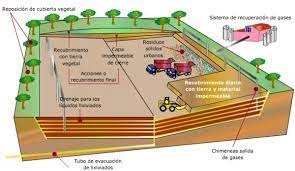
\includegraphics[width=4.16667in,height=\textheight]{desper.jpeg}

\begin{itemize}
\tightlist
\item
  Nuclear:La generación de energía nuclear implica la fusión de átomos
  de uranio o plutonio en un reactor nuclear para generar calor. Este
  calor se utiliza para producir vapor que mueve una turbina y genera
  electricidad. A diferencia de los combustibles fósiles, la energía
  nuclear no emite dióxido de carbono ni otros gases de efecto
  invernadero, lo que la convierte en una fuente de energía con bajas
  emisiones de carbono. Sin embargo, la energía nuclear también presenta
  riesgos, como la posibilidad de accidentes nucleares y la producción
  de residuos nucleares altamente peligrosos que deben ser almacenados
  durante cientos de miles de años. Debido a estos riesgos, la
  generación de energía nuclear es controvertida y se discute su
  seguridad y su impacto ambiental a largo plazo.
\end{itemize}

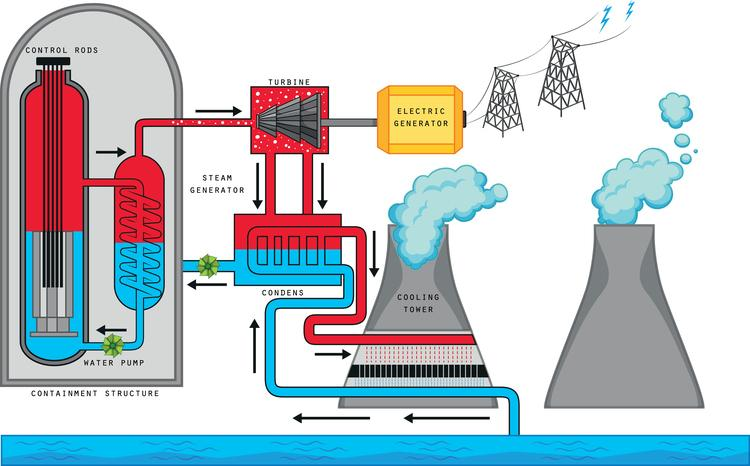
\includegraphics[width=4.16667in,height=\textheight]{nucle.jpeg}

\begin{itemize}
\tightlist
\item
  Hidro:La generación de energía hidroeléctrica implica la construcción
  de una presa para retener una gran cantidad de agua y liberarla de
  manera controlada a través de turbinas, generando energía mecánica que
  se transforma en electricidad mediante un generador. La energía
  hidroeléctrica es una forma de energía renovable y limpia que no emite
  gases de efecto invernadero ni otros contaminantes. Sin embargo, la
  construcción de presas y el represamiento de ríos pueden tener
  impactos significativos en el medio ambiente y la vida de las
  comunidades que dependen del río.
\end{itemize}

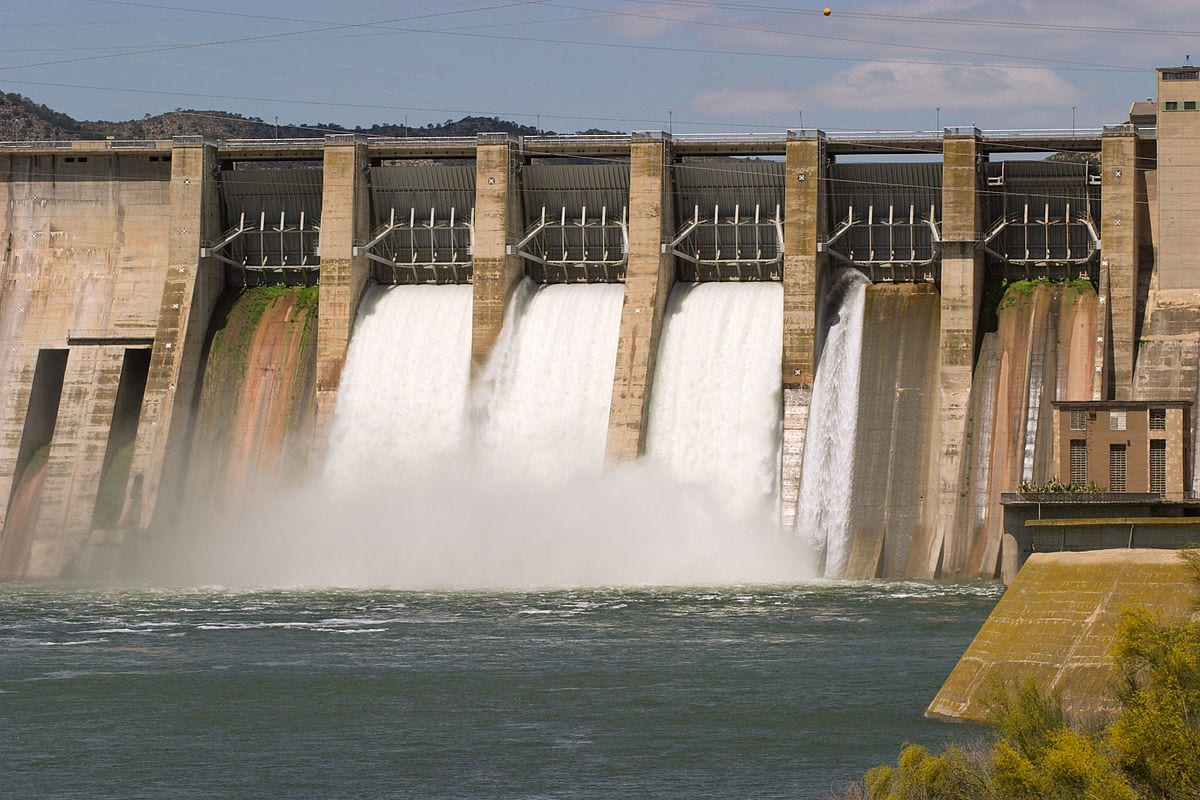
\includegraphics[width=4.16667in,height=\textheight]{hidro.jpeg}

\begin{itemize}
\tightlist
\item
  Geotermica:La generación de energía geotérmica consiste en la
  extracción de calor del interior de la Tierra a través de la
  perforación de pozos hasta llegar a reservorios de agua caliente y
  vapor en la corteza terrestre, y luego utilizar el vapor extraído para
  mover una turbina y producir electricidad. Es una fuente de energía
  renovable y limpia que no emite gases de efecto invernadero ni otros
  contaminantes, pero su construcción y operación pueden tener impactos
  ambientales y la disponibilidad de esta fuente de energía está
  limitada a ciertas regiones geográficas.
\end{itemize}

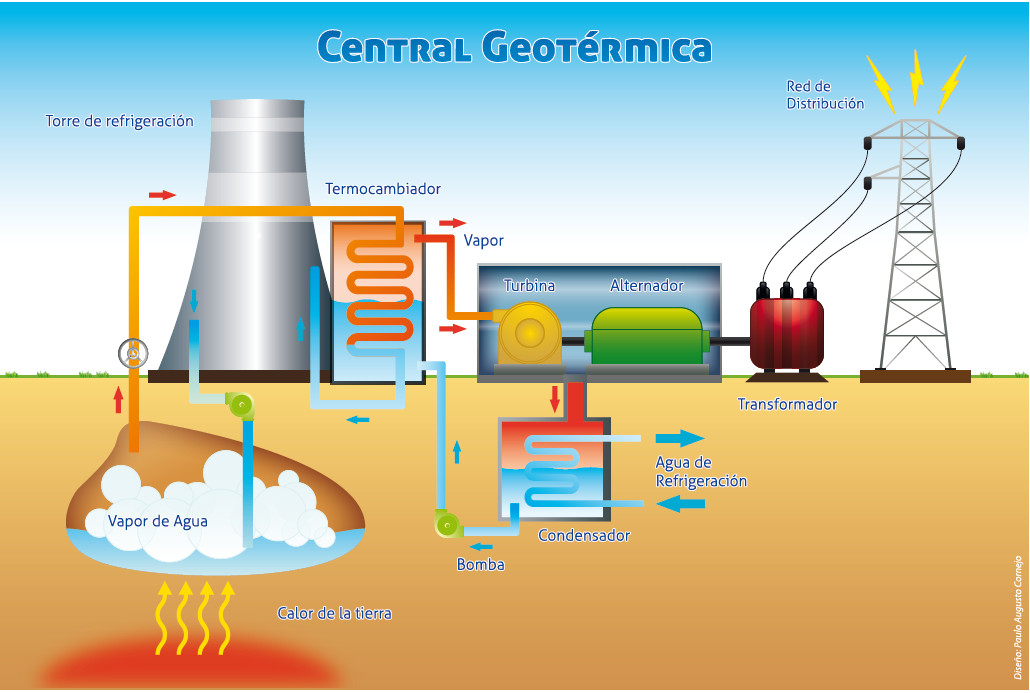
\includegraphics[width=4.16667in,height=\textheight]{geoter.jpeg}

\begin{itemize}
\tightlist
\item
  Energía Solar Fotovoltaica: La generación de energía solar
  fotovoltaica convierte la luz solar en electricidad utilizando paneles
  solares compuestos por celdas solares semiconductoras que liberan
  electrones cuando son expuestas a la luz. La energía solar es una
  fuente de energía renovable y limpia que no emite gases de efecto
  invernadero ni otros contaminantes, y su instalación en pequeña escala
  permite su uso en zonas remotas y en aplicaciones descentralizadas. No
  obstante, el costo inicial de instalación puede ser elevado y su
  eficiencia está limitada por factores como la intensidad de la luz
  solar y las condiciones climáticas.
\end{itemize}

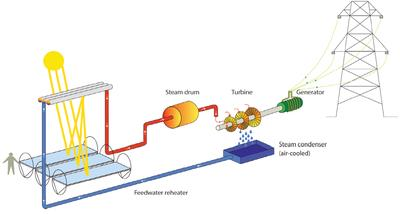
\includegraphics[width=4.16667in,height=\textheight]{fotovol.jpeg}

\begin{itemize}
\tightlist
\item
  Solar térmica: La generación de energía solar térmica se realiza a
  través de paneles solares que calientan un fluido, generalmente agua,
  para producir vapor y generar electricidad mediante una turbina. La
  energía solar térmica es una forma de energía renovable y limpia que
  no emite gases de efecto invernadero ni otros contaminantes en su
  proceso de generación, y es altamente eficiente en zonas con alta
  radiación solar. No obstante, su eficiencia está limitada por factores
  como la intensidad de la luz solar, la temperatura ambiente y la
  calidad de los materiales utilizados en los paneles solares térmicos.
\end{itemize}

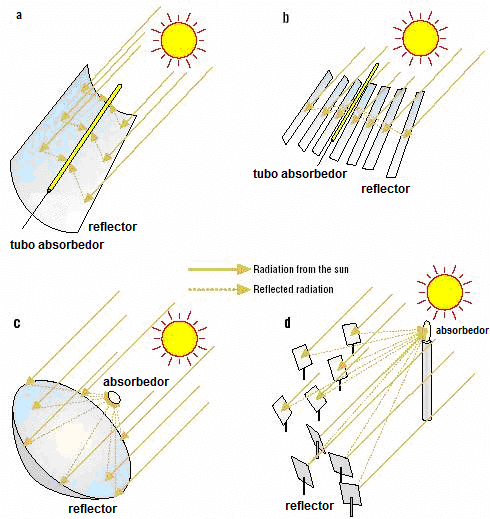
\includegraphics[width=4.16667in,height=\textheight]{termico.png}

\begin{itemize}
\tightlist
\item
  Viento: La generación de energía con viento implica la conversión de
  la energía cinética del viento en electricidad mediante el uso de
  turbinas eólicas. La energía eólica es una forma de energía renovable
  y limpia que no emite gases de efecto invernadero ni otros
  contaminantes en su proceso de generación, y es adecuada para su uso
  en zonas remotas o urbanas. Sin embargo, la eficiencia de la energía
  eólica está limitada por factores como la velocidad del viento y la
  ubicación geográfica de los parques eólicos.
\end{itemize}

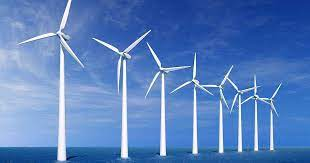
\includegraphics[width=4.16667in,height=\textheight]{viento2.jpeg}

\begin{itemize}
\tightlist
\item
  Mareas: La generación de energía con mareas se basa en la utilización
  de la energía cinética generada por el movimiento de las mareas para
  producir electricidad. La energía de las mareas es una forma de
  energía renovable y limpia que no emite gases de efecto invernadero ni
  otros contaminantes en su proceso de generación, y es predecible y
  constante. Sin embargo, la eficiencia de la generación de energía con
  mareas está limitada por la ubicación geográfica, ya que solo es
  viable en zonas cercanas al mar con grandes fluctuaciones en el nivel
  del agua.
\end{itemize}

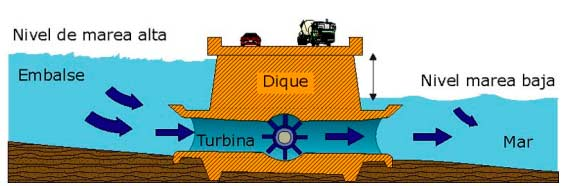
\includegraphics[width=4.16667in,height=\textheight]{mareas.jpeg}

Para llevar a cabo nuestro proyecto, en primera instacia contamos con
una base de datos la cual está conformada por 141 países y la
información presentada es la cantidad de energía que produce cada uno de
ellos a través de 12 medios de generación.

\begin{verbatim}
## # A tibble: 6 x 13
##   País    Coal    Oil    Gas Biofu~1 Waste Nuclear Hydro Geoth~2 Solar~3 Solar~4
##   <chr>  <dbl>  <dbl>  <dbl>   <dbl> <dbl>   <dbl> <dbl>   <dbl>   <dbl>   <dbl>
## 1 Alba~      0      0      0       0     0       0  5895       0       0       0
## 2 Alem~ 283710   6209  63017   44555 12824   91786 24898     134   38726       0
## 3 Alge~      0    908  67668       0     0       0   145       0      58       0
## 4 Ango~      0   4572      0       0     0       0  5193       0       0       0
## 5 Arab~      0 149537 188804       0     0       0     0       0       1       0
## 6 Arge~   3303  22357  71367    2138     0    7139 38529       0      15       0
## # ... with 2 more variables: Wind <dbl>, Tide <dbl>, and abbreviated variable
## #   names 1: Biofuels, 2: Geothermal, 3: `Solar PV`, 4: `Solar thermal`
\end{verbatim}

\hypertarget{normalizaciuxf3n}{%
\subsection{Normalización}\label{normalizaciuxf3n}}

La normalización es un proceso estadístico que se utiliza para escalar
valores en un conjunto de datos a una escala común. El objetivo de la
normalización es eliminar el efecto de la escala de las variables, para
que las variables estén en la misma escala y puedan ser comparadas de
manera justa.

Haciendo uso del mínimo y máximo podemos llevar un conjunto de datos a
una escala común. En este caso, los valores se escalan entre 0 y 1, de
manera que el valor mínimo en el conjunto de datos se convierte en 0 y
el valor máximo se convierte en 1. Su fórmula es:

\[Normalizacion=\frac{(x-min(x))}{max(x)-min(x)}\]

\begin{verbatim}
## Importance of components:
##                           PC1    PC2     PC3     PC4     PC5     PC6     PC7
## Standard deviation     0.3076 0.1366 0.12446 0.11526 0.08999 0.08772 0.07081
## Proportion of Variance 0.5580 0.1100 0.09138 0.07836 0.04778 0.04540 0.02958
## Cumulative Proportion  0.5580 0.6681 0.75943 0.83779 0.88557 0.93096 0.96054
##                            PC8     PC9    PC10    PC11    PC12
## Standard deviation     0.06263 0.03436 0.02850 0.02358 0.01474
## Proportion of Variance 0.02314 0.00696 0.00479 0.00328 0.00128
## Cumulative Proportion  0.98368 0.99065 0.99544 0.99872 1.00000
\end{verbatim}

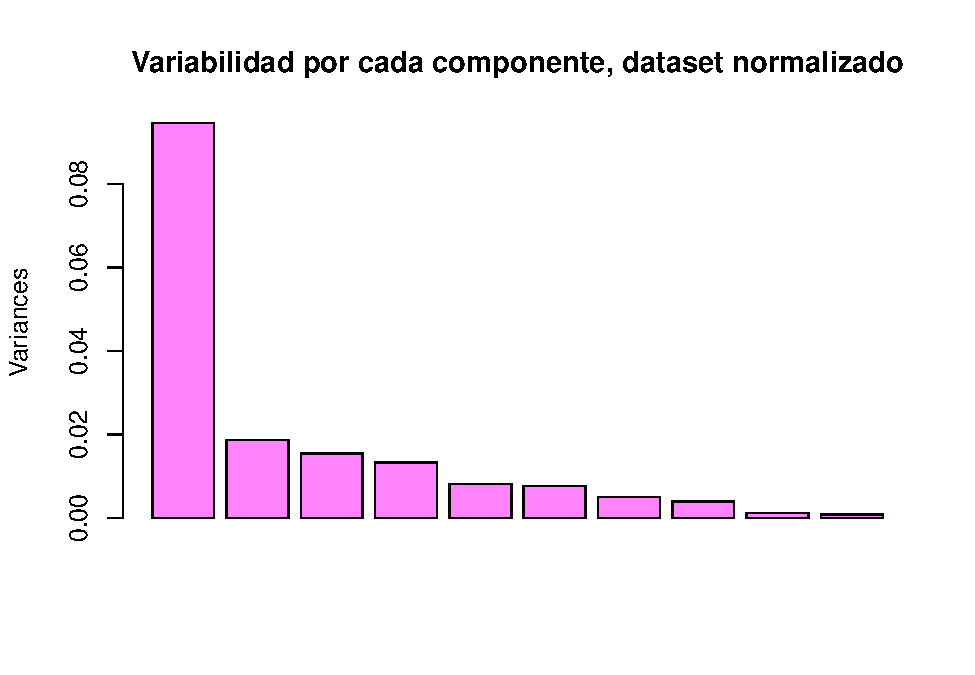
\includegraphics{AMTV_Docum_Consolidado_files/figure-latex/unnamed-chunk-11-1.pdf}

La normalización utilizando mínimo y máximo también se conoce como
``escalado entre 0 y 1''. Esta técnica es útil para comparar valores en
diferentes conjuntos de datos y para garantizar que las variables estén
en la misma escala antes de aplicar ciertas técnicas de análisis
estadístico, como la regresión y el análisis de componentes principales
(PCA).

\hypertarget{estandarizacion}{%
\subsection{Estandarizacion}\label{estandarizacion}}

La estandarización es un proceso estadístico que se utiliza para
transformar valores en un conjunto de datos de manera que tengan una
media de cero y una desviación estándar de uno. El objetivo de la
estandarización es eliminar el efecto de la escala y centrar los datos
en torno a cero, lo que permite comparar variables que tienen diferentes
unidades de medida.

La estandarización se realiza restando la media del conjunto de datos a
cada valor individual y dividiendo el resultado por la desviación
estándar. Esto tiene el efecto de ``centrar'' los datos en torno a cero
y de ``escalar'' los datos para que tengan una desviación estándar de
uno. Su fórmula es:

\[(Z)=\frac{x-\mu}{\sigma}\]

\begin{verbatim}
## Importance of components:
##                              PC1       PC2       PC3       PC4       PC5
## Standard deviation     3.976e+05 1.345e+05 4.892e+04 4.347e+04 1.461e+04
## Proportion of Variance 8.743e-01 1.001e-01 1.324e-02 1.045e-02 1.180e-03
## Cumulative Proportion  8.743e-01 9.744e-01 9.877e-01 9.981e-01 9.993e-01
##                              PC6       PC7       PC8       PC9  PC10  PC11
## Standard deviation     1.002e+04 4.112e+03 3.093e+03 1.723e+03 695.3 361.2
## Proportion of Variance 5.600e-04 9.000e-05 5.000e-05 2.000e-05   0.0   0.0
## Cumulative Proportion  9.998e-01 9.999e-01 1.000e+00 1.000e+00   1.0   1.0
##                         PC12
## Standard deviation     32.51
## Proportion of Variance  0.00
## Cumulative Proportion   1.00
\end{verbatim}

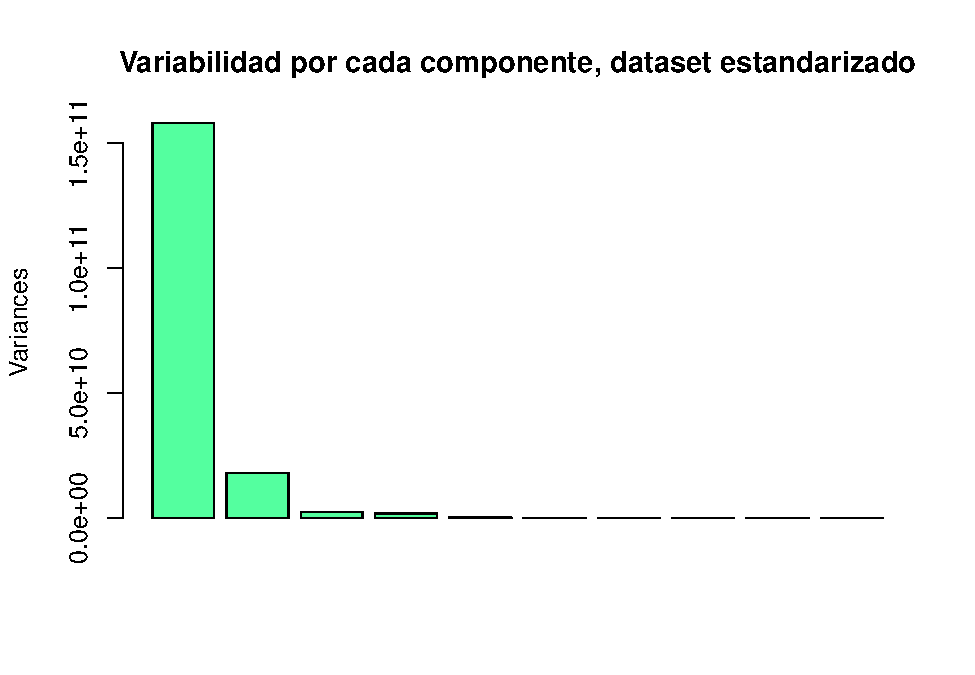
\includegraphics{AMTV_Docum_Consolidado_files/figure-latex/unnamed-chunk-13-1.pdf}

La estandarización es una técnica comúnmente utilizada en el análisis
estadístico para comparar variables que tienen diferentes unidades de
medida y para identificar valores extremos o atípicos en un conjunto de
datos. También se utiliza en la construcción de modelos estadísticos,
como el análisis discriminante y la regresión logística, donde las
variables deben estar en la misma escala para poder comparar sus efectos
en el modelo.

\hypertarget{porcentajes}{%
\subsection{Porcentajes}\label{porcentajes}}

La estandarización por medio de porcentajes es una técnica estadística
que se utiliza para comparar variables que están en diferentes escalas y
unidades de medida. En lugar de trabajar con los valores crudos de las
variables, la estandarización por medio de porcentajes convierte los
valores en porcentajes para que se puedan comparar de manera más
adecuada. Este método consiste en dividir cada un de los valores de la
variables entre el total de producción de energía:

\[Porcentajes=\frac{X_i}{Total}\]

La estandarización por medio de porcentajes es útil para comparar
variables que tienen diferentes unidades de medida, diferentes escalas o
diferentes magnitudes. Por ejemplo, se puede utilizar para comparar el
número de ventas de diferentes productos o marcas, o para comparar los
ingresos de diferentes empresas que operan en diferentes mercados o
regiones.

\begin{verbatim}
## Importance of components:
##                           PC1    PC2    PC3     PC4     PC5     PC6     PC7
## Standard deviation     0.3606 0.3238 0.3005 0.14789 0.07703 0.05577 0.03325
## Proportion of Variance 0.3638 0.2933 0.2525 0.06117 0.01659 0.00870 0.00309
## Cumulative Proportion  0.3638 0.6571 0.9096 0.97076 0.98735 0.99605 0.99914
##                            PC8      PC9     PC10      PC11      PC12
## Standard deviation     0.01605 0.006775 0.001698 9.624e-05 8.995e-17
## Proportion of Variance 0.00072 0.000130 0.000010 0.000e+00 0.000e+00
## Cumulative Proportion  0.99986 0.999990 1.000000 1.000e+00 1.000e+00
\end{verbatim}

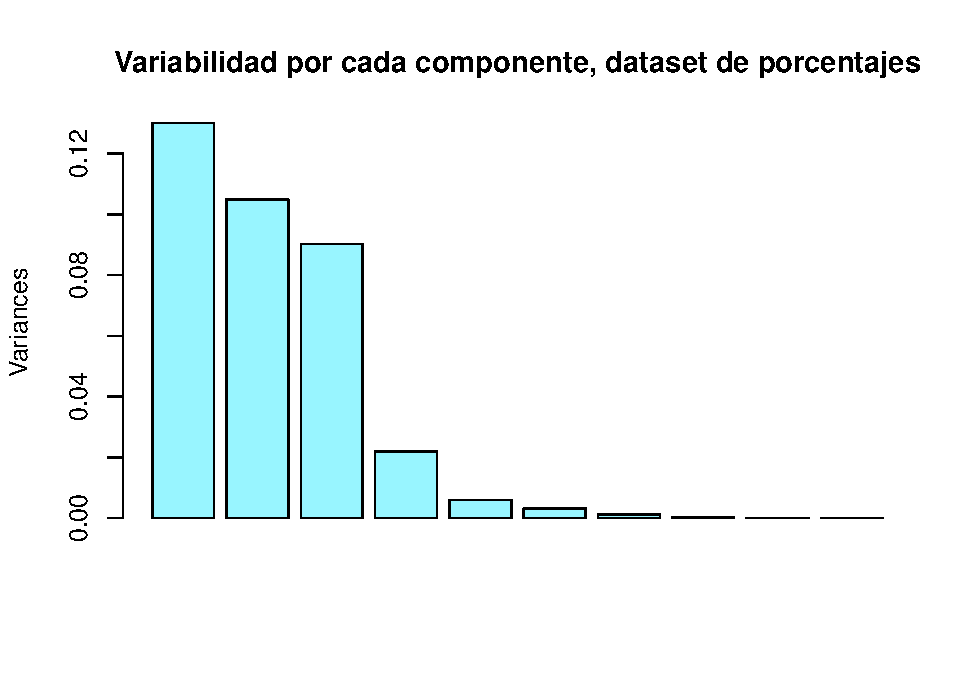
\includegraphics{AMTV_Docum_Consolidado_files/figure-latex/unnamed-chunk-16-1.pdf}

Finalmente, evidenciamos gráficamente el comportamiento de cada uno de
los distintos métodos utilizados para poder determinar cuál es la mejor
opción y llegar a conclusiones verídicas en cuanto a la generación de
energía.

\begin{verbatim}
##     normalizado estandarizado   porcentaje eje
## 1  0.0945907935  1.580627e+11 1.300647e-01   1
## 2  0.0186546352  1.809932e+10 1.048581e-01   2
## 3  0.0154903852  2.392989e+09 9.028661e-02   3
## 4  0.0132841899  1.889519e+09 2.187134e-02   4
## 5  0.0080988121  2.134094e+08 5.933165e-03   5
## 6  0.0076953742  1.004388e+08 3.110350e-03   6
## 7  0.0050142478  1.690800e+07 1.105612e-03   7
## 8  0.0039222870  9.569662e+06 2.577195e-04   8
## 9  0.0011805430  2.969192e+06 4.589837e-05   9
## 10 0.0008125279  4.834509e+05 2.883091e-06  10
## 11 0.0005559164  1.304680e+05 9.261536e-09  11
## 12 0.0002173683  1.056827e+03 8.091731e-33  12
\end{verbatim}

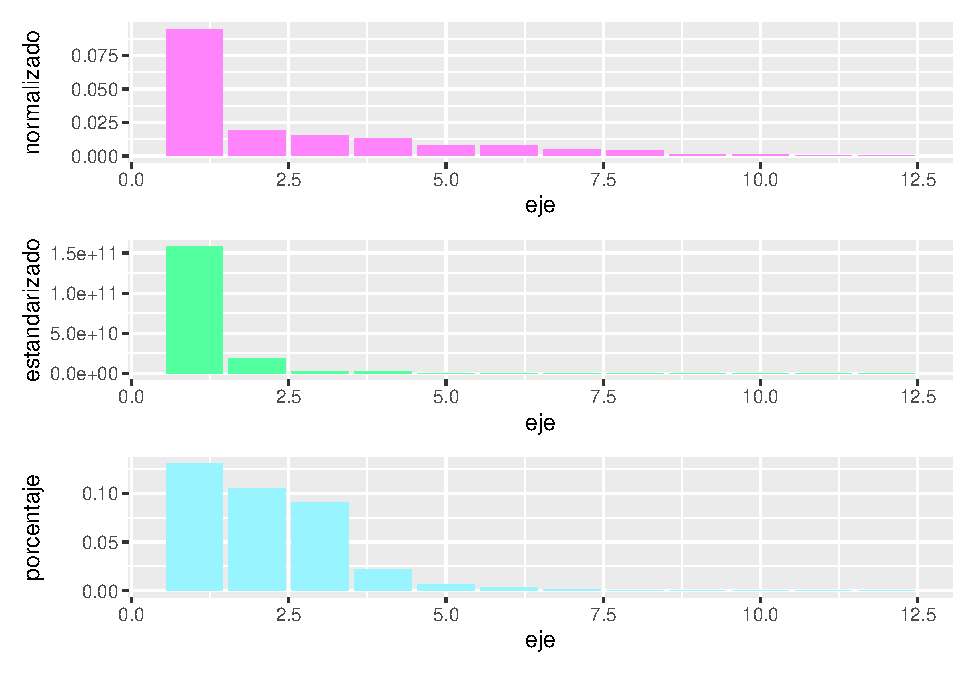
\includegraphics{AMTV_Docum_Consolidado_files/figure-latex/unnamed-chunk-18-1.pdf}

Seguido a esto, vamos a evaluar las correlaciones
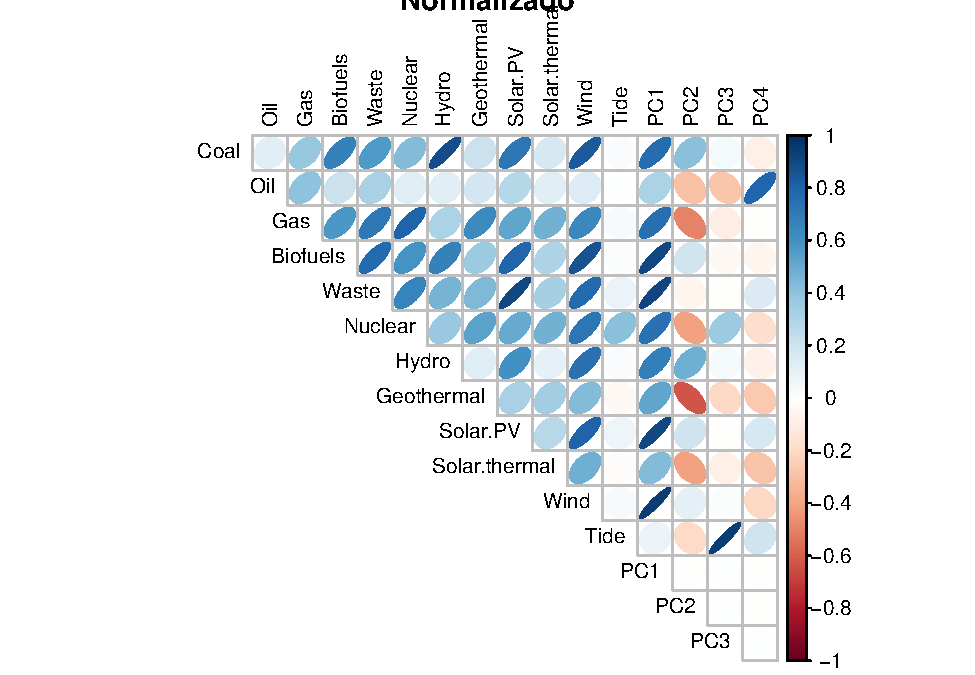
\includegraphics{AMTV_Docum_Consolidado_files/figure-latex/unnamed-chunk-19-1.pdf}

Evidenciamos que el 1 componente principal que se relaciona fuertemente
con oil, luego se relaciona con Geothermal y solar thermal,
posteriormente se relaciona con hydro, nuclear, gas y coal. Finalmente
se relaciona con biofuels, waste, solar.PV y Wind. Todas las relaciones
son positivas.

Evidenciamos que el 2 componente principal que se relaciona fuertemente
con coal, biofuels, solar.PV y Wind postivamente mientras que
negativamente se relaciona con Tide, nuclear, solar.themal luego y Oil,
por otro lado se relaciona con Geothermal, nuclear y gas negativamente,
mientras que positivamente hydro y coal.

Evidenciamos que el 3 componente principal que se relaciona fuertemente
con coal, hydro, wind y solar.PV positivamente, negativamente
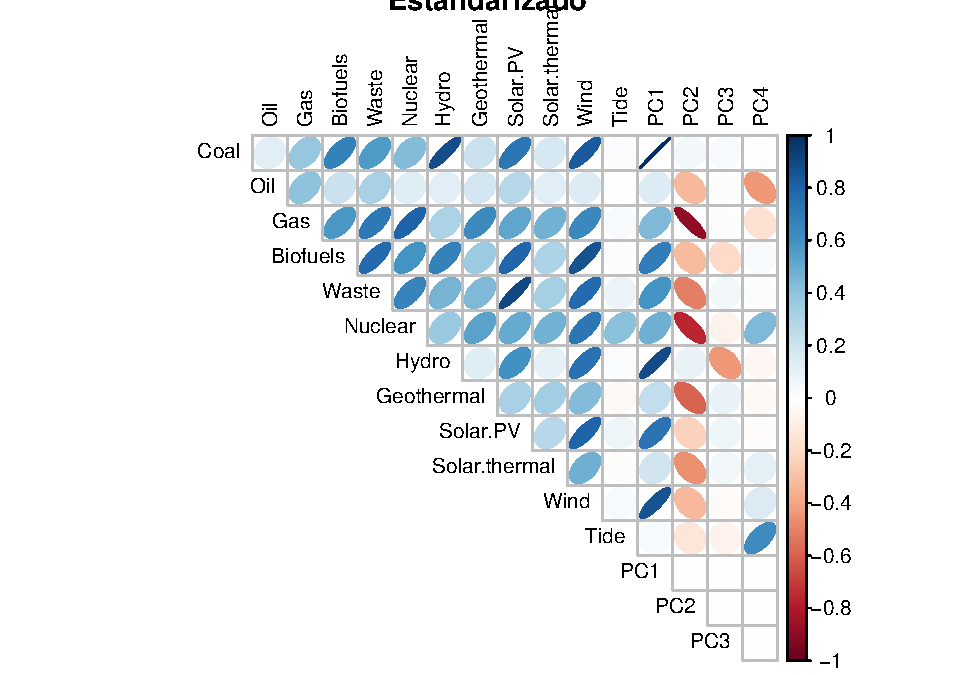
\includegraphics{AMTV_Docum_Consolidado_files/figure-latex/unnamed-chunk-20-1.pdf}
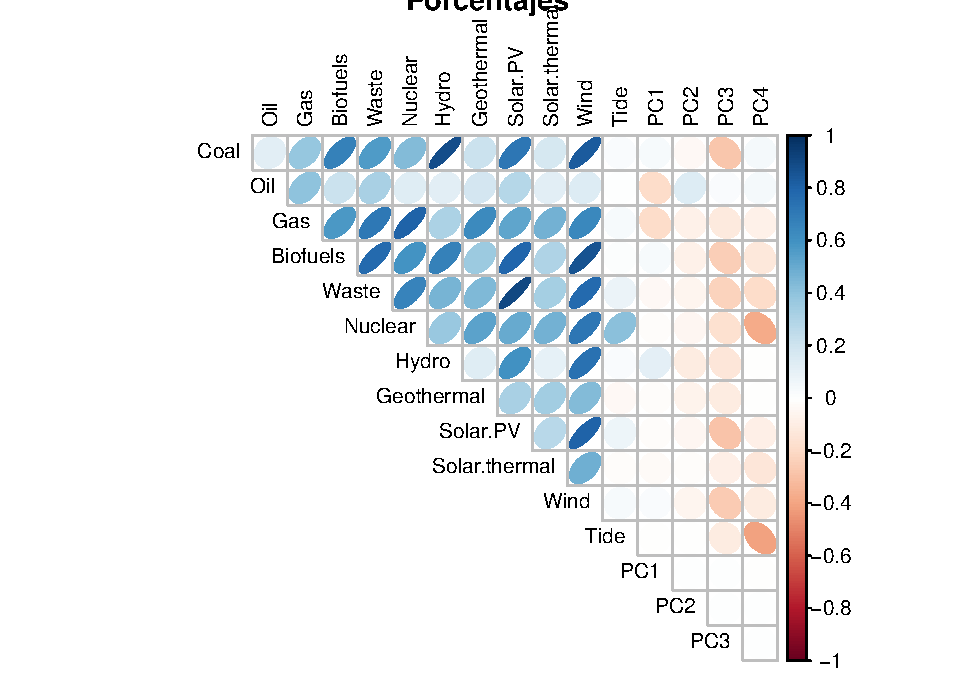
\includegraphics{AMTV_Docum_Consolidado_files/figure-latex/unnamed-chunk-20-2.pdf}

\end{document}
